\documentclass[aspectratio=169,10pt]{beamer}
\usetheme{Madrid}
\usecolortheme{default}
\usepackage{booktabs}
\usepackage{graphicx}
\graphicspath{{../results/}}
\setbeamertemplate{navigation symbols}{}
\newcommand{\TBD}{\textcolor{red}{TBD}}

\title[Herding outcome prediction]{Probabilistic Prediction of Outcome and Herding Time\\in Single-Pursuer Multi-Evader Herding}
\author{Shreyas}
\institute{EE604T Pattern Recognition and Machine Learning, IIT Dharwad}
\date{17 November 2026}

\begin{document}

\begin{frame}
\titlepage
\end{frame}

\begin{frame}{The problem in one picture}
\begin{columns}
\column{0.5\textwidth}
\begin{itemize}
\item One \textbf{pursuer} circles a goal; $N$ \textbf{evaders} run away from it (speed $k/d^2$).
\item The circle's radius follows the evader that was farthest at the start (arXiv 2505.10048).
\item Three things can happen:
  \begin{itemize}
  \item \textcolor{green!50!black}{\textbf{success}}: all evaders gathered on a small ring
  \item \textcolor{orange}{\textbf{deadlock}}: not settled within 300 laps
  \item \textcolor{red}{\textbf{loss}}: an evader escapes
  \end{itemize}
\item \textbf{Question:} from the start alone, predict the outcome, \emph{how sure} we are, and \emph{how long} herding takes.
\end{itemize}
\column{0.5\textwidth}
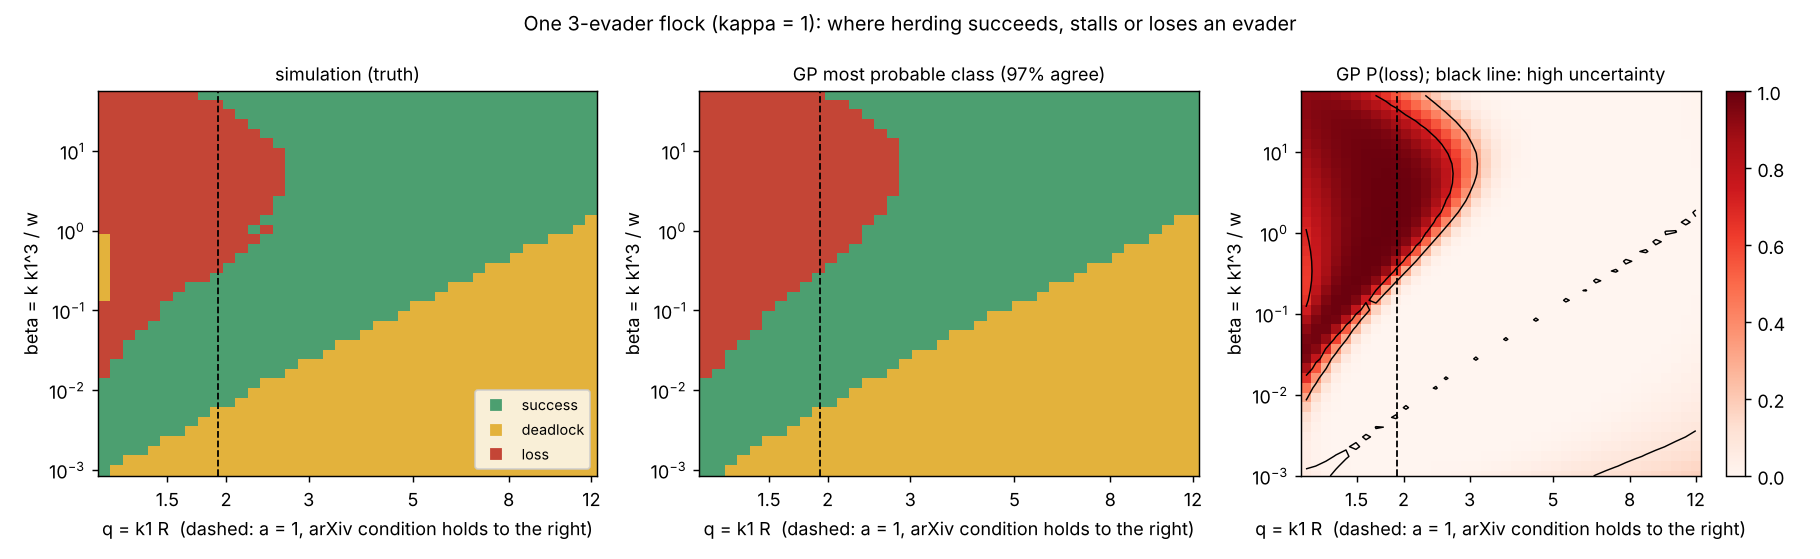
\includegraphics[width=\textwidth]{phase3/map.png}
\end{columns}
\end{frame}

\begin{frame}{Why machine learning? The theory is local}
\begin{itemize}
\item The papers prove a stable herd \emph{near the final ring} if $a = 2(k_1R)^2 e^{-2k_1\kappa} > 1$.
\item They say nothing about \emph{which starts} reach it, nor about time.
\item In our data the theorem rule is a poor predictor: \textbf{45.7\,\%} balanced accuracy.
  \begin{itemize}
  \item 52\,\% of successful runs violate $a>1$; 11\,\% of lost runs satisfy it.
  \end{itemize}
\item For the circle law, the paper's Lyapunov ellipse certifies only \TBD\ of the true success region.
\end{itemize}
\end{frame}

\begin{frame}{Data: 70{,}000 checked simulations}
\begin{itemize}
\item Own simulator; checked against both papers' numbers and an accurate solver: \textbf{700/700} identical labels.
\item Only two numbers matter after scaling: $q=k_1R$ and $\beta=kk_1^3/\omega$ (plus the start).
\item 60{,}000 arXiv-law runs, $N=1\ldots6$, three strata of $a$, Latin hypercube; 10{,}000 circle-law runs.
\item Labels: 26{,}454 success, 16{,}013 deadlock, 17{,}533 loss.
\item \textbf{Features} (24): describe only the start; do not depend on the evaders' order; work for any $N$.
\end{itemize}
\end{frame}

\begin{frame}{Classifiers: accuracy and honest probabilities}
\begin{columns}
\column{0.52\textwidth}
\small
\begin{tabular}{lcc}
\toprule
model (train runs) & bal.\ acc. & log-loss\\
\midrule
theory rule & 0.457 & --\\
logistic regression (48k) & 0.825 & 0.482\\
SVM + Platt (20k) & 0.938 & 0.200\\
\textbf{GP classifier (4k)} & \textbf{0.937} & \textbf{0.162}\\
\bottomrule
\end{tabular}
\vspace{2mm}
\begin{itemize}
\item Train $N\le4$, test $N=5,6$: \textbf{92.8\,\%}.
\item GP answers its 80\,\% most confident runs: \textbf{98.6\,\%}.
\item Bayes rule (losing an evader costs most): "loss called success" 169 $\to$ \textbf{9}.
\end{itemize}
\column{0.48\textwidth}
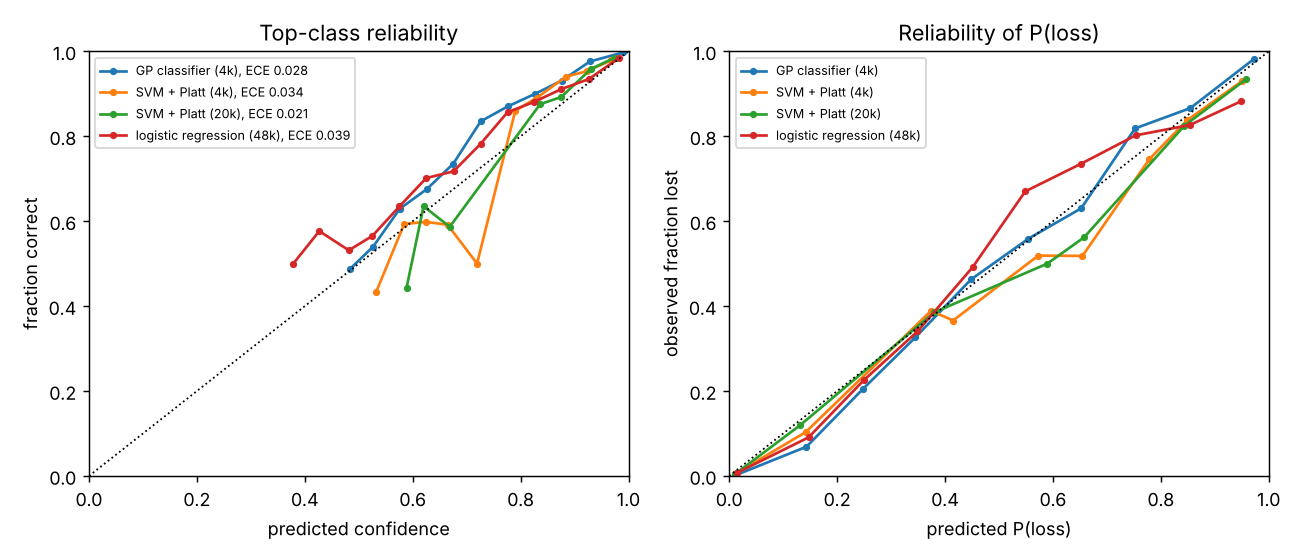
\includegraphics[width=\textwidth]{phase3/reliability.png}
\end{columns}
\end{frame}

\begin{frame}{Novelty 1: risk-aware active learning}
\begin{itemize}
\item Simulations cost time: let the GP \textbf{choose the next simulation}.
\item \emph{Entropy}: where the model is unsure. \emph{Risk-aware} (ours): where a wrong decision costs most.
\end{itemize}
\centering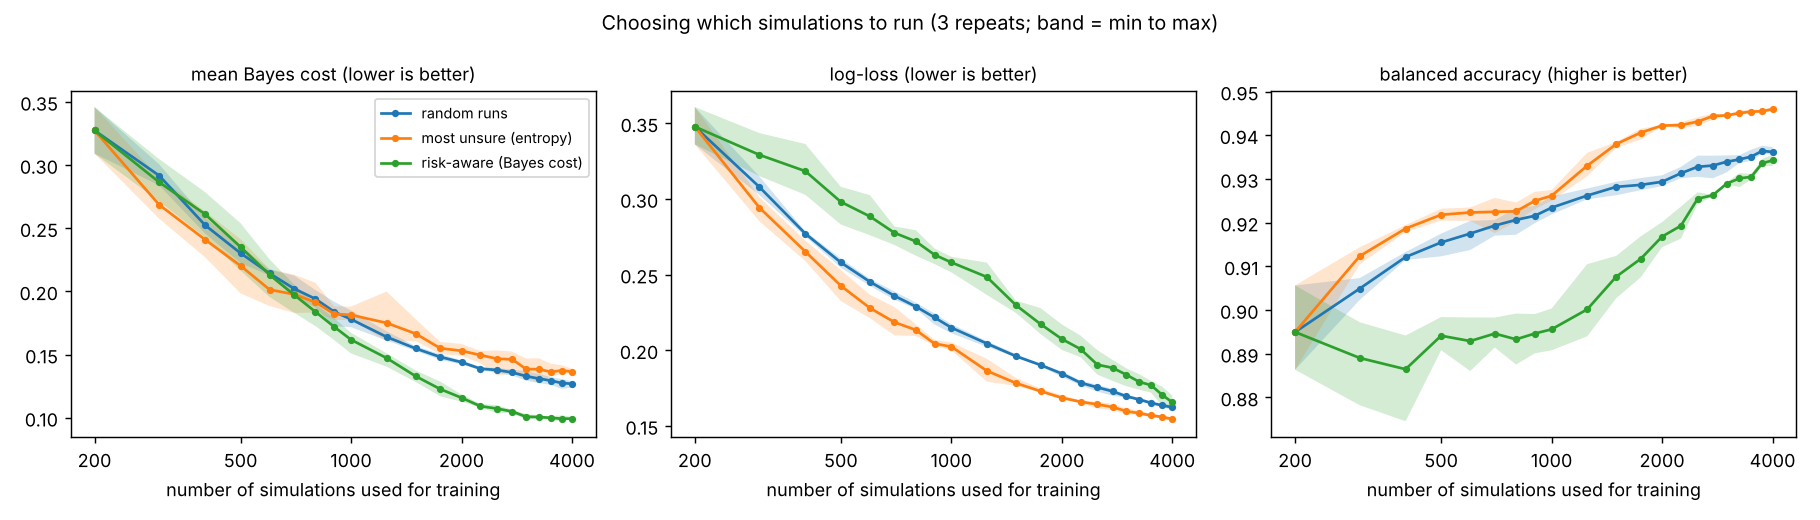
\includegraphics[width=0.85\textwidth]{novelty/active.png}
\begin{itemize}
\item Risk-aware: same decision cost as random with \textbf{2.3$\times$ fewer} runs; entropy: best accuracy but \emph{worse} decisions.
\end{itemize}
\end{frame}

\begin{frame}{Novelty 2: herding time with censoring (slow vs stuck)}
\begin{itemize}
\item Deadlock runs only tell us "time $>$ 300 laps". Dropping them biases the model.
\item Kernel \textbf{mixture-cure} survival model: $P(\text{ever settles})$ + time if it settles.
\item Check: 300 deadlock runs re-simulated \textbf{10$\times$ longer}: \TBD.
\end{itemize}
\centering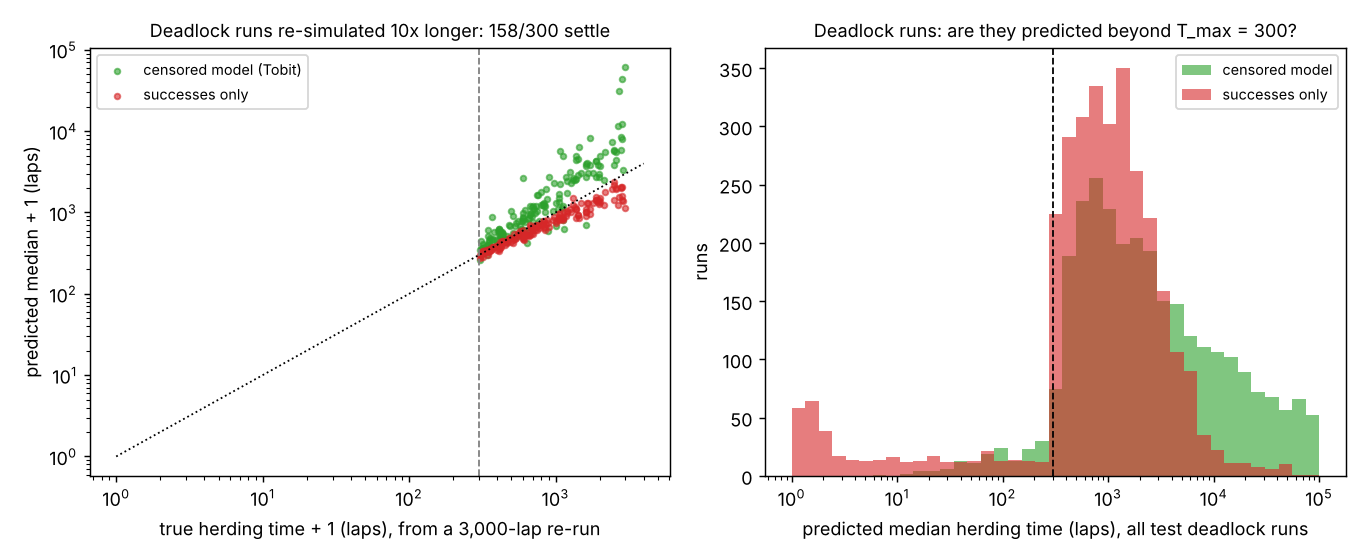
\includegraphics[width=0.75\textwidth]{censored/censored.png}
\end{frame}

\begin{frame}{Novelty 3: using the model to choose the pursuer settings}
\TBD
\end{frame}

\begin{frame}{Do the regimes appear without labels? (GMM + PCA)}
\centering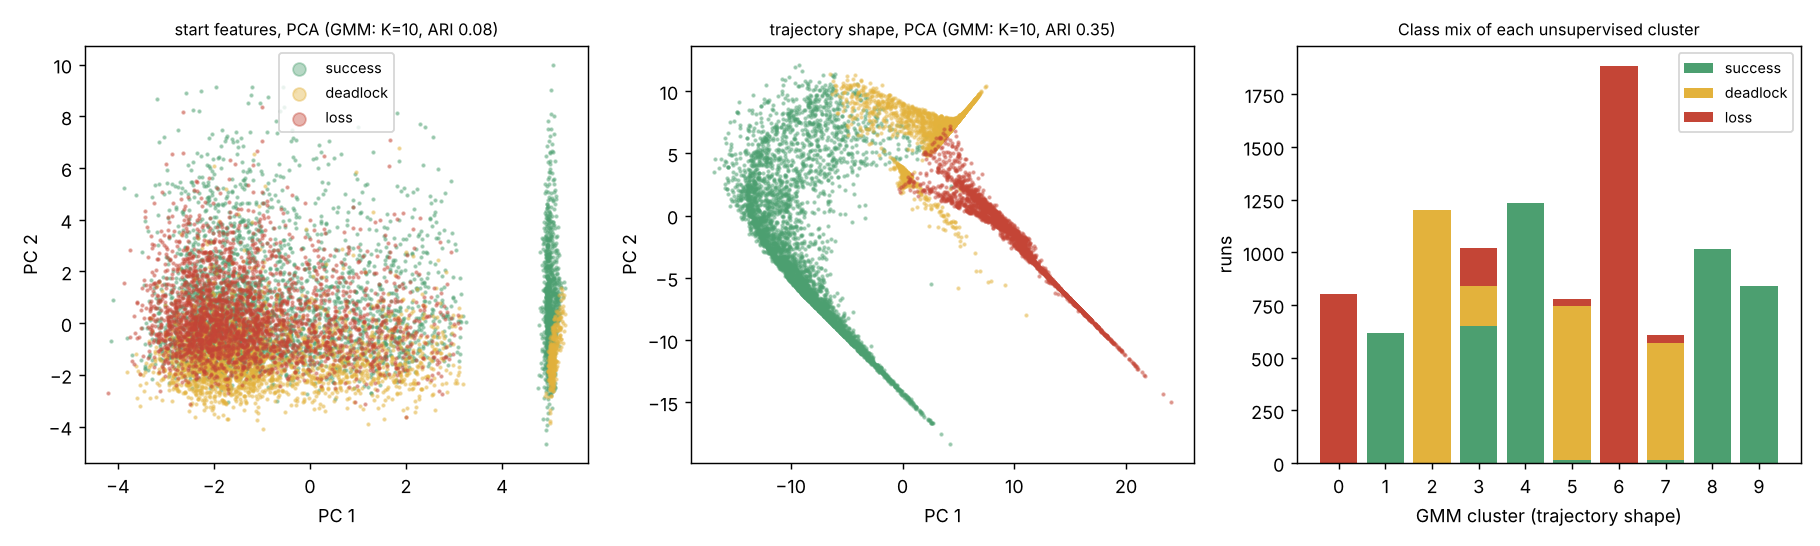
\includegraphics[width=0.95\textwidth]{regimes/regimes.png}
\begin{itemize}
\item From the start: no (ARI 0.08) $\Rightarrow$ supervision is needed.
\item From the trajectory shape: three arms, clusters \textbf{95\,\% pure} $\Rightarrow$ the labels are natural regimes.
\end{itemize}
\end{frame}

\begin{frame}{Set kernel: compare flocks as sets of points}
\TBD
\end{frame}

\begin{frame}{Theory vs data: the circle law}
\TBD
\end{frame}

\begin{frame}{Honest limits}
\begin{itemize}
\item Everything is simulation; labels depend on our numbers ($T_{\max}=300$ laps, 1\,\%).
\item Exact GP limited to 4{,}000 training runs ($O(n^3)$); kernel tuned on 1{,}000.
\item The cost matrix is a design choice.
\item Active learning chooses from a pool of already-simulated runs (equivalent here: the simulator is deterministic).
\end{itemize}
\end{frame}

\begin{frame}{Summary}
\begin{itemize}
\item Calibrated, uncertainty-aware prediction of outcome and herding time, for any flock size.
\item Shows where the local theory stops protecting the evaders.
\item Censored survival model separates slow from stuck herds.
\item Risk-aware active learning: choose simulations by the decision you will make.
\item Live demo: set up a flock $\to$ probabilities, decision, time $\to$ simulate and compare.
\end{itemize}
\end{frame}

\end{document}
